\documentclass{amsart} 
\usepackage{graphicx}
\graphicspath{{./}}
\usepackage[fontsize=14pt]{scrextend}
\usepackage{hyperref}
\usepackage{csvsimple}
\usepackage{epigraph}
\title{Human Nature Is 75,000 Years Old}
\author{Zulfikar Moinuddin Ahmed}
\date{\today}
\begin{document}
\maketitle
\epigraph{
Oh go and tell the king 

that the sky is falling in

It's the devil's way now

There is no way out

You can scream and you can shout

It is too late now}{Radiohead, "2+2=5"}

\section{Introduction}
Human Nature theories have developed in the East and the West over the millenia by Ancient and modern philosophers, and there has been a great deal of work in the past century.  We want to consider Human Nature in terms of evolutionary history of the Human Race.  This is a moment of confusion regarding Human Race because we have not overcome the errors of the past theorists and the primitive beliefs of multiple races of human beings have not been completely eliminated.  

We do know today with quite fair confidence that the non-African populations of Earth all had ancestors in a single meta-tribe of Africa 75,000 years ago.  I will not address genetic evidence for this.  

\section{Human Nature is dated 75,000 years in the past}
Philosophers like to think in terms of concepts that are abstract and universal and use methods of thought to determine various features of truth about things.  Neither Ancient nor more modern philosophers before the twentieth century had any access to the knowledge of genome that we possess today.  One has to remember that the discovery of DNA itself was announced in 1953 by Watson and Crick, and all study of human genetic history is obviously subsequent.  

We know that non-Africans of Earth had ancestors in a single tribe in East Africa around 75,000 years ago.  We can thus conclude that Human Nature consists of the characteristics of this meta-tribe.  

\section{Inference: Human Nature difficult to fathom}

We cannot simply note down behaviour patterns of people in daily life and determine Human Nature easily.  This nontriviality of Human Nature is easy to understand for what is common among non-Africans today is buried in 75,000 years of genetic evolutionary history and therefore the expression of this human nature is not necessarily easy to decipher from overt behaviour.  

This inference gives us some appreciation for the difficult ambition of the philosophers Ancient and modern who attempted to theorize regarding Human Nature at all, for they had taken on a deep challenge of understanding what is possibly latent and subtle from 75,000 years of history in our genome.

\section{Inference: Human Nature is rich and complex}

Human Nature as the characteristics of a single meta-tribe in East Africa 75kya represents previous evolution of 6 million years, which means that the commonality is highly complex and rich and not reducible to features of pre-human primate behaviour.  

I want to quickly consider the great work of Steven Pinker in his books such as {\it The Blank Slate}.  John Locke had theorized the human mind as a blank slate and over time cognitive psychologists had shown that there are large numbers of evolutionary adaptations that provide mind with many features that are not learned but inherited.  

Blank slate hypothesis is wrong along with many other speculative hypotheses formulated by many thinkers both in East and West over the past centuries.  

\section{Human Nature Focus on 75kya gives concreteness}

We want to find some concrete time and genetic and behavioural core that can allow us to form the core of our understanding of Human Nature, and my time scale proposition will give more than research direction.  It will allow human societies to understand some hidden drivers to our behaviour that is just long enough ago as to require careful study rather than superficial self-evident behaviour.

\section{Non-Arbitrariness}

These are simple points but worth making very clear because the proposition is to consider the Human Nature not arbitrary but concrete.  In common vernacular and informal language we might mean by 'human nature' a generalized idea of how we are which could be so unspecific as to be meaningless.  We choose 75kya because this is the peak of development that allowed dispersal of our ancestors West and East.

\section{Africans}
I want to point out explicitly that Human Nature for African peoples in my estimate is exactly the same as non-Africans and so there is no hidden motive here except that non-Africans differ superficially enough to make the substance of the difficulty of Human Nature in the ancestral meta-tribe of Africans.

\section{Mapping My Human Nature with Common Usage}
The extreme focus of East Africans 75kya is my proposal for Human Nature.  Their gene pool is one that contains the commonality of non-Africans.  Africans did not differ much from the dispersing meta-tribe and so Human Nature is universal.

\section{Human Nature is to be Happy when Social and Respect Needs are Met}

Tay and Diener looked at well-being across the globe and their measurements show remarkable stability of psychological Social and Respect need correlation with Subjective Well-Being.

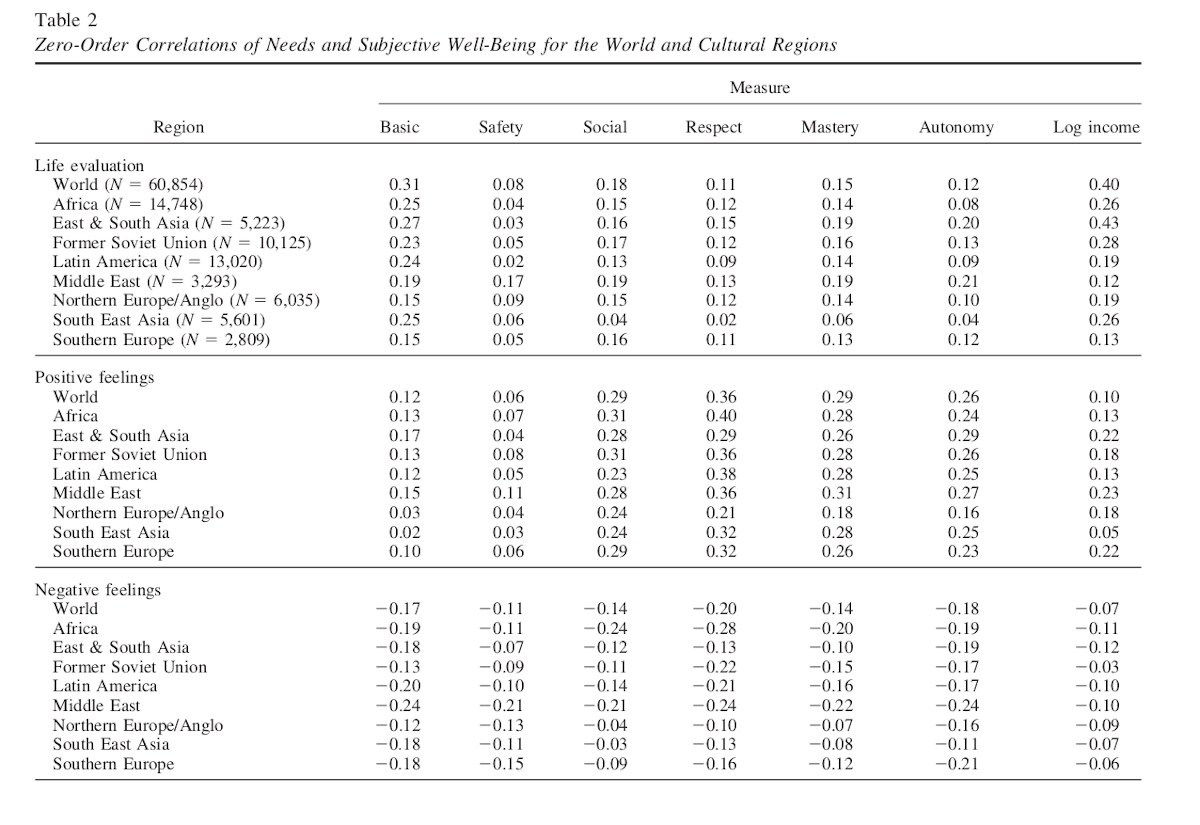
\includegraphics[scale=0.35]{wbneeds.png}

Examination of the figures will show you this.  Thus Social and Respect needs are strong components of Human Nature.  I have argued elsewhere that seventeenth and eighteenth century Western thinkers had concentrated on selfishness and altruism as dichotomy for Human Nature but in fact the population statistics showed that these both vary over the global population with 20\% altruistic and 80\% selfish and therefore neither is human nature fundamentally.  On the other hands Human Nature includes Social and Respect {\em needs} because the stability across the globe of their effects on Positive Feelings part of Well-Being.

\end{document}
